\section{Maze and multi-agent exploration}
\label{section_models_maze}
For simulation purposes, this work modeled a maze under a 4-neighbor 2D grid graph perspective, where each cell is a square with its edges composed by a wall or not. If there is a wall, an agent cannot traverse the maze across the related edge. On the other hand, if there is not a wall, an agent has a free way to traverse the maze through the related edge. It is worth to mention that, if an edge has a wall, the edge of the adjacent corresponding cell also has necessarily a wall.

The maze has a goal that is a single marked cell, and an agent inside the maze aims to find the marked cell, traversing the maze cell by cell. This agent is an autonomous entity that follows a specific algorithm according the current explored path and its programmed initial rules. So that it doesn't go through the same path more than one time, it stores the visited cells. Thus, when there are various posible branches to extend the agent's path, it ignores cells already visited by itself, and, if there is not a candidate to be a possible branch, the agent go back to the previous visited cell. Furthermore, specifically to this research, differently from some approaches presented in \citen{Beisel2014}, \citen{Burgard2005}, and \citen{KivelevitchCohen2010}, there is no intercommunication between agents in a multi-agent situation to solve the maze.

\citen{Muhammad2021} developed an open-source maze generator. It is a python module that creates randomly mazes and enables the user to simulate its own maze-solving algorithm. In this context, this work presents a multi-agent maze-solving algorithm that has been simulated over \citen{Muhammad2021} open-source code, with modifications. Figure \ref{maze_model} presents, for example, 2 agents traversing a $6 \times 6$ maze toward the goal.

\citen{Muhammad2021} software creates by default a ``perfect maze'', which means that there is one and only one path to the goal from any cell. However, it is possible to set the code to generate a imperfect maze.

\begin{figure}[ht!]
\centering
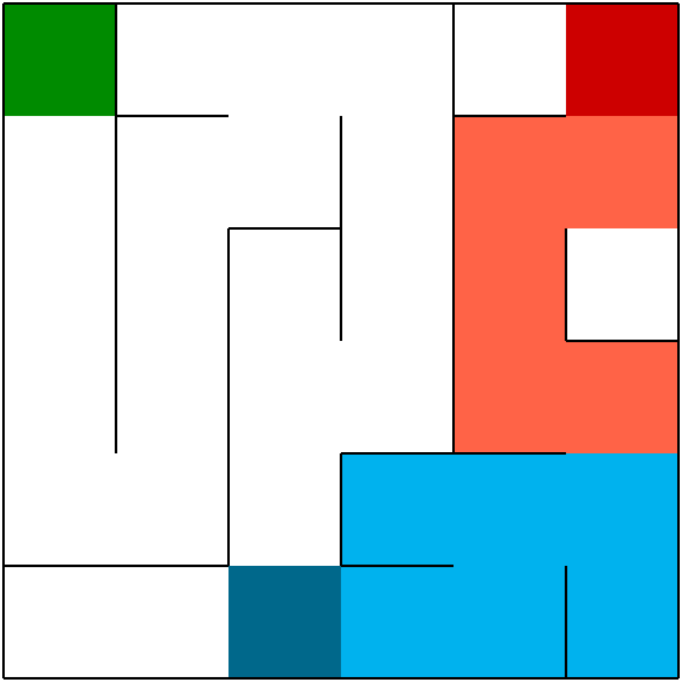
\includegraphics[width=0.5\textwidth]{Cap2/maze_model.png}
\caption{Blue and red agents traversing a $6\times 6$ maze. The goal is represented by the green entity. This maze is a perfect maze \cite{Muhammad2021}.}
\label{maze_model}
\end{figure}

\section{Maze from a graph topology perspective}
\label{section_models_maze_graph}
As pointed out in Section \ref{section_models_maze}, given that an agent ignores visited cells, there are important statements related to this work:

\begin{itemize}
\item if there is only one path to the goal from any cell, it is valid to consider a maze as a tree, i.e., a perfect maze \cite{Muhammad2021};

\item if there is more than one path to the goal from any cell, the maze cannot be considered as a tree, but it might be considered as a general 2D grid;

\item despite the last statement, and also considering that an agent ignores visited cells, an agent path always might be individually interpreted as a tree.
\end{itemize}

Figure \ref{maze_example_graph} gives an example of the graph representation of the maze presented in Figure \ref{maze_example}, where a red agent is traversing the maze toward the green goal. As established by \citen{Muhammad2021}, the maze cells are programmatically addressed as indices of a matrix, such as represented in Figure \ref{maze_indices_muhammad}.

\begin{figure}[ht!]
\centering
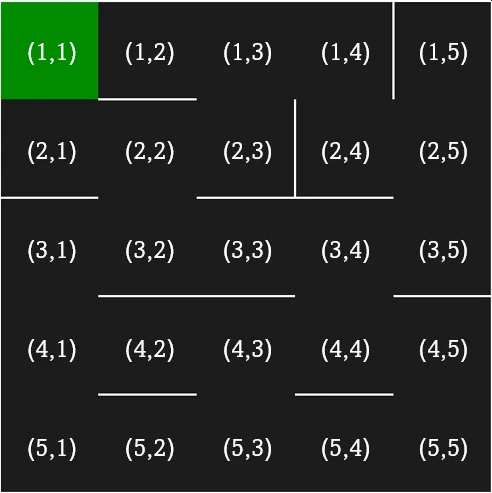
\includegraphics[width=0.5\textwidth]{Cap2/maze_indices_muhammad.png}
\caption{Maze cell indices. Source: \citen{Muhammad2021}.}
\label{maze_indices_muhammad}
\end{figure}

\begin{figure}[ht!]
\centering
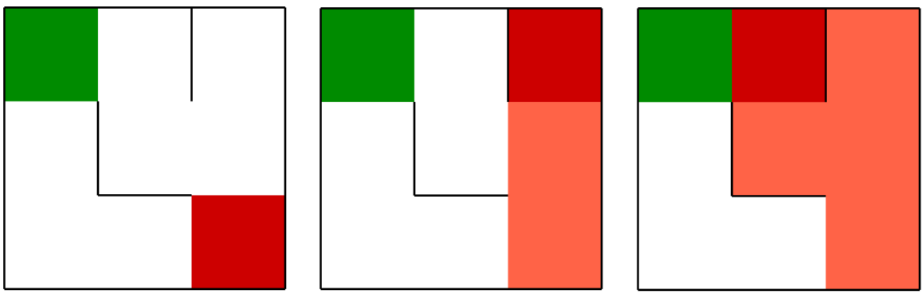
\includegraphics[width=0.7\textwidth]{Cap2/maze_example.png}
\caption{Red agent traversing a maze toward the green goal. This maze is not a perfect maze.}
\label{maze_example}
\end{figure}

\begin{figure}[ht!]
\centering
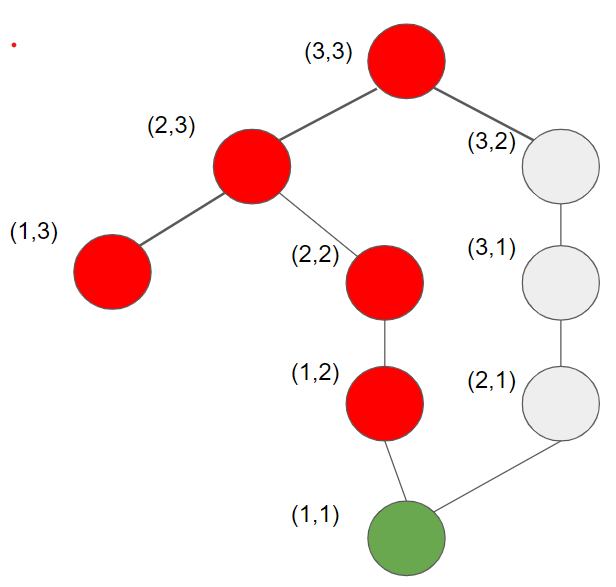
\includegraphics[width=0.5\textwidth]{Cap2/maze_example_graph.png}
\caption{Graph representation of the maze presented in Figure \ref{maze_example}. The cell indices are pointed out, and the cells visited by the red agent are also pointed out.}
\label{maze_example_graph}
\end{figure}	

\section{Multi-agent exploration without communication}
\label{section_models_exploration}
The goal of this work is to present a maze-solving algorithm in a multi-agent environment, where an agent cannot communicate with the other agents. Thus, each agent must be previously programmed to avoid exploring the same portion of the maze as other agents. Indeed, they should be as dispersed as possible.

First of all, this research considers a maze as a graph, where each node is a cell representation of the maze. Given a initial node that the agent starts its path through it, the agent checks if the node has children. Supposing that a node of the graph has at least one child, i.e., there are not completely walled cells, important statements are established:

\begin{itemize}
\item if an agent finds the node where is the goal, the agent finishes its path;

\item if an agent is not in the node where is the goal and the node has only one child, the agent necessarily goes through this node child;

\item if an agent is not in the node where is the goal and the node has more than one child, the agent needs to decide to which child it will move itself.
\end{itemize}

To establish an decision algorithm to the last statement, this work proposes firstly a interval division related to the agents and the children. Supposing that there are $k$ agents $a_{1}, a_{2},...,a_{k}$ to explore the maze, each agent will have a corresponding and proportional range of action related to the graph, as presented below:

\begin{equation}
	\begin{align}
			d = 1/k\\
		a_{1} \textnormal{: } [0, d[\\
		a_{2} \textnormal{: } [d, 2d[\\
		a_{3} \textnormal{: } [3d, 4d[\\
		...\\
		a_{k} \textnormal{: } [(k-1)d, 1]
	\end{align}
\end{equation}
where $d$ is the size of the partition corresponding to each agent. On the other hand, this work has handled convergence intervals to each node, where the agents tends to match its interval with the node convergence interval. In this way, an agent intends to traverse the maze as dispersed from the others as possible.

As pointed out in Section \ref{section_definitions_graph}, a graph may be represented as an adjacency list. Given that an agent path through an unknown maze may be represented as a tree, and considering the agent path as an adjacency list $A$, where the first explored node (root) $v_{1}$ has a convergence interval equal to $[0,1]$, while the other nodes $v_{i}$ of the maze are unknown, i.e., the agent doesn't know previously their convergence intervals, Pseudocode \ref{pseudocode_1} establishes the convergence intervals of each node. As mentioned previously, there is no communication between agents, therefore each agent needs to explore the maze individually, and calculates by itself the convergence intervals of each node. Furthermore, it is important to emphasize that each agent considers individually the maze as tree, where the root is the agent's starting node.

\begin{algorithm}
\caption{Traverse of the agent through the maze (interpreted as a tree by the agent)}
\label{pseudocode_1}
\begin{algorithmic}
%\Require $n \geq 0$
%\Ensure $y = x^n$

\State $agent\_interval \gets [a_{min},a_{max}]$ \hspace{0.5cm} \slash\slash \hspace{0.1cm} Previously defined interval of the agent

\State $current\_node \gets v_{1}$ \hspace{1cm} \slash\slash \hspace{0.1cm} Agent starts the exploration at node $v_{1}$

\State $visited\_nodes \gets [$ $]$ \hspace{0.95cm} \slash\slash \hspace{0.1cm} Array of visited nodes by the agent is initially empty

\State $intervals[v_{1}$] $\gets [0,1]$ \hspace{0.65cm} \slash\slash \hspace{0.1cm} $v_{1}$ is the root

%\State $A [0][0] \gets 0$ \hspace{2.35cm} \slash\slash \hspace{0.1cm} adjacency list $A$ is initially $1 \times 1$

\State $A \gets \oslash$ \hspace{3.1cm} \slash\slash \hspace{0.1cm} Initialize the empty adjacency list of the tree $A$

\State $complete(A, v_{1})$ \hspace{1.55cm} \slash\slash \hspace{0.1cm} In the tree $A$, create a list for $v_{1}$ and complete the list of
\State \hspace{4.45cm} \slash\slash \hspace{0.1cm} $v_{1}$ with the children of $v_{1}$. The order of insertion of child
\State \hspace{4.45cm} \slash\slash \hspace{0.1cm} must follow some rule. In the case of this work, the inser-
\State \hspace{4.45cm} \slash\slash \hspace{0.1cm} tion is clockwise (North, East, South, West)\\

\\

\textbf{while} $current\_node$ is not the goal cell \textbf{do}\\

\hspace{0.3cm} \textbf{if} $current\_node$ is not in $visited\_nodes$ \textbf{then}\\

\hspace{0.6cm} $append(visited\_nodes, current\_node)$\\

%\hspace{0.6cm} $max \gets \max \{intervals[current\_node]\}$\\

\hspace{0.6cm} $max \gets get\_maximum\_value(intervals[current\_node])$\\

%\hspace{0.6cm} $min \gets \min \{intervals[current\_node]\}$\\

\hspace{0.6cm} $min \gets get\_minimum\_value(intervals[current\_node])$\\

\hspace{0.6cm} $partition \gets (max - min) \slash amount\_of\_children$\\

\hspace{0.6cm} $count \gets 0$\\

\hspace{0.6cm} \textbf{foreach} child $v_{j}$ of $current\_node$ in $A$ \textbf{do}\\

\hspace{0.9cm} $intervals[v_{j}] \gets [min + count \cdot  partition, min + (count+1) \cdot  partition[$\\

\hspace{0.9cm} $complete(A, v_{j})$\\

\hspace{0.9cm} $count \gets count + 1$\\

\hspace{0.6cm} \textbf{end foreach}\\

\hspace{0.3cm} \textbf{end if}\\

\hspace{0.3cm} \textbf{if} $current\_node$ has no child \textbf{or} all of $current\_node$'s children were visited \textbf{then}\\

\hspace{0.6cm} $current\_node \gets get\_parent(A, current\_node)$\\

\hspace{0.6cm} \textbf{continue}\\

\hspace{0.3cm} \textbf{end if}\\

\hspace{0.3cm} \textbf{foreach} child $v_{j}$ of $current\_node$ in $A$ \textbf{do}\\

\hspace{0.6cm} \textbf{if} $v_{j}$ is in $visited\_nodes$ \textbf{then}\\

\hspace{0.9cm} \textbf{continue} \\

\hspace{0.6cm} \textbf{else}\\

\hspace{0.9cm} $max\_node \gets get\_maximum\_value(interval[v_{j}])$\\

\hspace{0.9cm} $min\_node \gets get\_minimum\_value(interval[v_{j}])$\\

\hspace{0.9cm} $max\_agent \gets get\_maximum\_value(agent\_interval)$\\

\hspace{0.9cm} $min\_agent \gets get\_minimum\_value(agent\_interval)$\\

\hspace{0.9cm} \textbf{if} $min\_agent < max\_node$ \textbf{then}\\

\hspace{1.2cm} \slash\slash \hspace{0.1cm} This condition only works because the order of children is well defined\\
\hspace{1.2cm} $current\_node \gets v_{j}$\\

\hspace{1.2cm} \textbf{break} \\

\hspace{0.9cm} \textbf{end if}\\

\hspace{0.6cm} \textbf{end if}\\

\hspace{0.3cm} \textbf{end foreach}\\

\hspace{0.3cm} \slash\slash \hspace{0.1cm} If \textit{current\_node} remains the same as the beginning of the iteration, it means\\

\hspace{0.3cm} \slash\slash \hspace{0.1cm} that the agent finished its interval, and then it needs to change its behavior. \\

\hspace{0.3cm} \slash\slash \hspace{0.1cm} Then its behavior is domain dependent. It will continue the DFS under some\\

\hspace{0.3cm} \slash\slash \hspace{0.1cm} criteria  \\

\hspace{0.3cm} \textbf{if} $current\_node$ remains the same as the beginning of the \textit{while} iteration \textbf{then}\\

\hspace{0.6cm} $current\_node \gets continue\_DFS\_under\_some\_criteria(A, current\_node)$\\

\hspace{0.3cm} \textbf{end if}\\

\textbf{end while}
\end{algorithmic}
\end{algorithm}}

Figure \ref{maze_example_graph_intervals} presents the converge intervals of the nodes if at least two agents explored the maze presented in Figure \ref{maze_example} using Pseudocode \ref{pseudocode_1}.

Thus, the goal of this work aims to establish an efficient algorithm that interrelates the agent intervals to the maze node intervals. Furthermore, the authors observed that a mixed radix representation to the agent path is a powerful mathematical tool to relate the path to the interval of the node that the agent is visiting, and it will be present in the next report.

\begin{figure}[ht!]
\centering
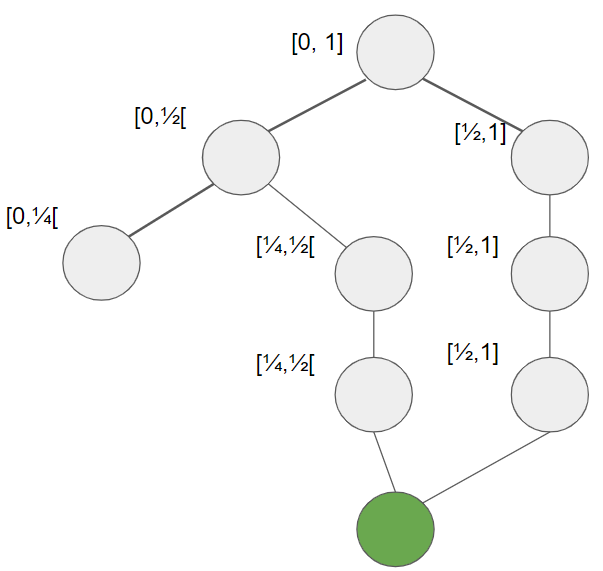
\includegraphics[width=0.5\textwidth]{Cap2/maze_example_graph_intervals.png}
\caption{Graph representation of the maze presented in Figure \ref{maze_example}, with intervals related to the agent's range of action.}
\label{maze_example_graph_intervals}
\end{figure}	

\section{Mixed radix representation to the agent path}
\label{section_models_mixed_radix}
In Section \ref{section_models_exploration}, this work presented a method to an agent traverse the maze by defining ranges of action, despite it needs some improvements. Pseudocode \ref{pseudocode_1} explain this method, and establishes a way to explore the maze while an agent records the visited nodes and the explored tree. However, the agent doesn't need in fact to save the tree, because it only needs to know the current node interval to make a decision.

This work establish a method to 